% UPC 2023 A 中文修订稿；现有单栏排版，XeLaTeX。
\documentclass[11pt,a4paper]{article}
\usepackage[UTF8,scheme=plain,fontset=windows]{ctex}
\usepackage[margin=25mm,headheight=16pt]{geometry}
\usepackage{lmodern}
\usepackage{microtype}
\usepackage{amsmath,amssymb,booktabs,graphicx,float,tabularx,array}
\usepackage[section]{placeins}
\usepackage[font=small,labelfont=bf]{caption}
\usepackage{fancyhdr,lastpage}
\usepackage{hyperref}
\usepackage{xurl}
\hypersetup{colorlinks=true,linkcolor=black,urlcolor=blue,citecolor=black,
 pdftitle={太空跳伞的下降过程、危险性与最大出舱高度},pdfsubject={UPC 2023 问题 A 中文修订稿}}
\setlength{\parindent}{2em}
\setlength{\parskip}{0.25em}
\pagestyle{fancy}\fancyhf{}
\fancyhead[L]{UPC 2023 \quad 问题 A：Space Diving}
\fancyhead[R]{第 \thepage\ 页，共 \pageref{LastPage} 页}
\fancyfoot[C]{\thepage}
\renewcommand{\headrulewidth}{0.4pt}
\renewcommand{\contentsname}{目录}
\renewcommand{\refname}{参考文献}
\renewcommand{\figurename}{图}
\renewcommand{\tablename}{表}
\newcolumntype{Y}{>{\raggedright\arraybackslash}X}
\renewenvironment{abstract}{}{}
\newcommand{\keywords}[1]{\noindent\textbf{关键词：}#1}
\newcommand{\FitArea}{1.3570}
\newcommand{\MaxHeight}{58.22}
\newcommand{\PeakV}{608.5}
\newcommand{\PeakMach}{1.999}
\newcommand{\FreeG}{2.54}
\newcommand{\OpenG}{4.42}
\newcommand{\SpinG}{0.071}
\newcommand{\LandingV}{5.50}
\newcommand{\TotalTime}{664.6}
\newcommand{\FreeTime}{245.0}
\newcommand{\ChuteTime}{419.6}
\newcommand{\CanopyArea}{66.50}
\newcommand{\CanopyB}{99.75}
\newcommand{\OpenV}{70.28}
\newcommand{\Tzero}{419.5}
\newcommand{\OctV}{340.7}
\newcommand{\OctError}{9.66}
\newcommand{\CurveRMSE}{22.68}
\newcommand{\CurveMAE}{16.29}
\newcommand{\CurveBias}{-15.67}
\newcommand{\CurveMax}{53.33}
\newcommand{\Energy}{2.87}
\newcommand{\Stroke}{0.386}
\newcommand{\FirstSonic}{34.19}
\newcommand{\LastSonic}{101.80}
\newcommand{\SuperTime}{67.61}
\newcommand{\HeightConvergence}{0.0056}
\newcommand{\FastOpenG}{6.49}
\newcommand{\FastOverTime}{0.666}
\newcommand{\MinimumInflation}{6.37}
\newcommand{\SixtyHeatTime}{16.74}
\newcommand{\SeventyHeatTime}{39.25}
\newcommand{\EightyHeatTime}{47.87}

\begin{document}
\thispagestyle{empty}
\begin{center}
{\Large\bfseries 太空跳伞的下降过程、危险性与最大出舱高度}\\[10pt]
{\normalsize The 2023 University Physics Competition · Problem A}\\[16pt]
{\large\bfseries 摘要}
\end{center}

\begin{abstract}
针对总质量为190\,kg的跳伞者、压力服及降落伞系统，本文建立覆盖自由下降、姿态运动、有限时间开伞和伞降着陆的连续动力学模型，求解典型装备条件下的最大出舱高度。以《1976年美国标准大气》的七层温度梯度为基础，通过位势高度变换、静力平衡及理想气体状态方程构造温度、压力和密度的分段表达式；采用2017年Stratos研究的三段马赫数阻力系数，并对其适用范围以上的部分作常值延拓。利用2012年3月和7月跳跃峰速，在固定阻力系数0.6、参考质量121.2\,kg的条件下，联合标定迎风面积为\FitArea\,m$^2$，随后将该面积用于190\,kg工况。

10月跳跃用于检验面积迁移，模型峰速为\OctV\,m/s，较公开值377.1\,m/s低\OctError\%。从2017年原图提取411个速度—高度点后，共同高度区间的均方根误差为\CurveRMSE\,m/s。本文保留这一偏差，并指出阻力公式本身来自10月飞行，因此该比较属于同源模型检验。姿态部分采用含恢复力矩、偏置力矩与气动阻尼的两自由度角运动方程；热分析采用恢复温度及滞止温度；开伞部分将人体阻力与平滑增长的伞衣阻力相加。

在恢复温度不超过400\,K、自由下降与开伞气动过载均不超过5\,$g_0$、头部径向载荷不超过2\,$g_0$、着陆速度不超过6\,m/s的典型设计条件下，8\,s充气方案得到最大出舱高度约\MaxHeight\,km。该工况峰速为\PeakV\,m/s，峰值马赫数为\PeakMach，自由下降过载为\FreeG\,$g_0$，开伞过载为\OpenG\,$g_0$，着陆速度约\LandingV\,m/s，全程约\TotalTime\,s。恢复温度是中心情景的主导限制；将其设计上限改为380--420\,K，最大高度相应变为55.21--61.18\,km。4\,s充气的峰值过载增至\FastOpenG\,$g_0$，高偏置力矩情景也可产生很大的旋转载荷。因此，约58\,km是本文所选装备和姿态条件下的建模答案，开伞控制、姿态稳定和热防护共同决定其可行性。

\end{abstract}
\medskip
\keywords{太空跳伞；分层大气；迎风面积标定；气动加热；姿态运动；有限充气}
\newpage
{\small\tableofcontents}
\newpage

\section{引言}
\subsection{研究背景}
高空跳伞把人体直接置于稀薄、低压的大气环境中。出舱初期空气阻力很小，下降速度迅速增加；进入较稠密的大气后，阻力和气动力矩增强，人体经历减速、气动加热及姿态调整，随后还需完成开伞与着陆。随着出舱高度提高，这几个阶段的危险会以不同方式变化，单独考察峰值速度不足以判断能否成功下降。

2012年的Red Bull Stratos计划留下了多次高空跳跃的高度、峰速、低过载持续时间和开伞记录\cite{summit}。Guerster与Walter进一步研究了10月飞行的跨声速阻力特征，给出了随马赫数变化的阻力系数\cite{guerster}。这些数据为面积标定和模型检验提供了依据，也说明人体的姿态与不规则外形会影响跨声速气动特性。

\subsection{问题陈述与分析}
UPC 2023问题A设定：火箭将一名穿着压力服、携带降落伞的人竖直送至高空，总质量为190\,kg，出舱后下降至地面，要求分析挑战、危险及最大可成功下降的高度\cite{problem}。本文把火箭释放点视为相对大气瞬时静止的位置，以海平面为着陆面，并选取一组可明确计算的装备与姿态条件。

求解分为三个相互衔接的任务：首先建立随高度变化的大气环境与气动力，利用历史跳跃确定迎风面积；其次将平移、角运动、热指标和开伞过程联系起来，计算各阶段的极值及持续时间；最后在出舱高度范围内搜索同时满足多项设计约束的可行区间。质量、面积和阻力系数分别进入动力学方程，避免将不同质量和姿态的跳跃直接按同一减速规律处理。

\section{模型假设}
\begin{enumerate}
\item 出舱时相对无风大气的竖直速度为零，轨迹近似竖直。忽略水平漂移、地球自转、升力及火箭尾流；大气性质仅随高度变化。
\item 系统总质量恒为190\,kg。压力服保持密封并提供足够的供氧与压力支持，生命保障持续时间覆盖所求下降时间。此项是进入动力学分析的装备前提。
\item 标准大气模型限制在几何高度0--86\,km，采用常气体常数和完全气体近似。空气温度梯度取自原始标准文献，未用外推温度层扩展到更高处。
\item 自由下降的中心姿态为腹部朝下。标定面积在190\,kg工况保持相同；质量增加由装备承载，不额外改变中心外形。俯仰扰动通过投影面积改变阻力。
\item 人体与装备近似刚体。姿态采用俯仰和绕下降轴平旋两个自由度，使用固定参考惯量，忽略两轴之间的陀螺耦合及人体主动动作；参数代表典型稳定构型。
\item 主伞在几何高度2566.8\,m开始充气；较低出舱情景在释放时立即开始充气。伞降阶段假设姿态已稳定、伞绳无缠绕、伞衣完整。开伞高度沿用公开跳跃记录的海拔量级，着陆面另设为海平面。
\item 热风险以恢复温度上限筛选。压力服的实际表面温度与人体温度需要额外传热参数，本模型不将两者等同于气流热指标。
\end{enumerate}

表\ref{tab:design}明确区分经验输入与设计选择。载荷采用$g_0=9.80665$\,m/s$^2$归一化；在自由下降和开伞阶段均以气动力产生的加速度定义过载。NASA的人体系统设计资料强调加速度耐受与方向、持续时间及约束方式有关\cite{hidh}，因此本文采用的5\,$g_0$是情景筛选值。后续同时改变阈值和姿态参数，以评估答案对这些选择的依赖。
\begin{table}[htbp]\centering\small
\caption{中心情景的主要输入及其性质}\label{tab:design}
\begin{tabularx}{\linewidth}{p{38mm}p{34mm}Y}\toprule
参数 & 中心取值 & 依据或含义\\\midrule
总质量$m$ & 190\,kg & 题目给定\\
标定参考质量 & 121.2\,kg & 2017年论文式17\cite{guerster}\\
迎风面积$A$ & \FitArea\,m$^2$ & 3月、7月峰速联合标定\\
开伞高度$h_o$ & 2566.8\,m & 峰会报告的海拔记录\cite{summit}\\
充气时间$\tau$ & 8\,s；对照4\,s & 有限充气设计情景\\
海平面平衡伞降速度 & 5.5\,m/s & 参考伞具下降速度量级，重新配置面积\\
自由段、开伞过载上限 & 各5\,$g_0$ & 典型设计条件，扫描4--6\,$g_0$\\
恢复温度上限 & 400\,K & 热设计筛选值，扫描380--420\,K\\
头部径向载荷上限 & 2\,$g_0$ & 历史载荷量级对照，扫描1--3\,$g_0$\\
着陆速度上限 & 6\,m/s & 与5.5\,m/s平衡设计值留有裕量\\\bottomrule
\end{tabularx}
\end{table}

\section{符号说明}
主要符号列于表\ref{tab:symbols}。高度向上为正，下降速度$v$向下为正；角速度保留旋转方向的符号，径向载荷取其幅值。
\begin{table}[htbp]\centering\small
\caption{主要符号与单位}\label{tab:symbols}
\begin{tabularx}{\linewidth}{p{27mm}Y>{\raggedright\arraybackslash}p{28mm}}\toprule
符号 & 含义 & 单位\\\midrule
$h,h_0,h_o$ & 几何高度、出舱高度、开伞高度 & m\\
$z,x$ & 位势高度；$x=z/(1000\,\mathrm m)$ & m；无量纲\\
$t,v,g$ & 时间、向下速度、当地重力加速度 & s；m/s；m/s$^2$\\
$R_e,R$ & 参考地球半径、空气比气体常数 & m；J/(kg\,K)\\
$T,p,\rho$ & 大气温度、压力、密度 & K；Pa；kg/m$^3$\\
$T_i,p_i,\rho_i,L_i$ & 第$i$层底部量及温度梯度 & K；Pa；kg/m$^3$；K/m\\
$c,M,C_D$ & 声速、马赫数、人体阻力系数 & m/s；1；1\\
$A,A_{\rm eff},q,D$ & 标定面积、投影面积、动压、人体阻力 & m$^2$；m$^2$；Pa；N\\
$c_p,\Pr,r_T$ & 定压比热、普朗特数、恢复系数 & J/(kg\,K)；1；1\\
$T_{\rm aw},T_0$ & 恢复温度、滞止温度 & K\\
$\theta,\psi,\omega_p,\omega_z$ & 俯仰角、平旋角及对应角速度 & rad；rad/s\\
$I_p,I_z,B_\omega$ & 两轴惯量、气动角阻尼系数 & kg\,m$^2$；N\,m\,s\\
$C_\theta,C_n,C_\omega$ & 恢复、偏置及角阻尼的无量纲系数 & 1\\
$A_c,C_{D,c},B_c$ & 等效伞面积、伞阻力系数及其乘积 & m$^2$；1；m$^2$\\
$S,\tau,n_D,n_o,n_r$ & 充气函数、充气时间及三类归一化载荷 & 1；s；1\\\bottomrule
\end{tabularx}
\end{table}

\section{模型建立}
\subsection{地球大气层}
\subsubsection{高度变换与温度分层}
《1976年美国标准大气》印刷页3表4采用七段位势温度梯度\cite{ussa}。取$R_e=6\,356\,766$\,m，几何高度与位势高度的关系为
\begin{equation}
 z=\frac{R_eh}{R_e+h},\qquad h=\frac{R_ez}{R_e-z},\qquad
 \frac{\mathrm dz}{\mathrm dh}=\left(\frac{R_e}{R_e+h}\right)^2.
 \label{eq:height}
\end{equation}
几何高度86\,km对应$z=84.85205$\,km，表中末界面按原文精度记为84.852\,km。定义$x=z/(1000\,\mathrm m)$，七段温度（单位K）写为
\begin{equation}
T(x)=\begin{cases}
288.15-6.5x,&0\le x<11,\\
216.65,&11\le x<20,\\
216.65+(x-20),&20\le x<32,\\
228.65+2.8(x-32),&32\le x<47,\\
270.65,&47\le x<51,\\
270.65-2.8(x-51),&51\le x<71,\\
214.65-2(x-71),&71\le x\le84.85205.
\end{cases}\label{eq:temperature}
\end{equation}
七层的底部状态列于表\ref{tab:layers}。原文温度表使用分子标度温度；本文采用常分子量近似，将其用于声速和理想气体关系。80--86\,km的分子量修正未单独处理，这一近似位于所求中心高度以上。

\begin{table}[htbp]\centering\small
\caption{七层位势区间、温度梯度与递推得到的层底状态}\label{tab:layers}
\begin{tabular}{rrrrrr}\toprule
层 & $z$区间/km & $L_i$/(K/km) & $T_i$/K & $p_i$/Pa & $\rho_i$/(kg/m$^3$)\\\midrule
\input generated/layers.tex 
\bottomrule\end{tabular}
\end{table}

\subsubsection{由静力平衡求压力和密度}
令$R=287.05287$\,J/(kg\,K)，采用随高度变化的重力
\begin{equation}
 g(h)=g_0\left(\frac{R_e}{R_e+h}\right)^2.
 \label{eq:gravity}
\end{equation}
静力平衡及理想气体关系为
\begin{equation}
 \frac{\mathrm dp}{\mathrm dh}=-\rho g(h),\qquad p=\rho RT,
 \qquad \frac{\mathrm dp}{\mathrm dz}=-\frac{g_0p}{RT(z)}.
 \label{eq:hydro}
\end{equation}
因此，在第$i$层，$T=T_i+L_i(z-z_i)$，从层底积分得到
\begin{equation}
 p(z)=\begin{cases}
 p_i[T(z)/T_i]^{-g_0/(RL_i)},&L_i\ne0,\\
 p_i\exp[-g_0(z-z_i)/(RT_i)],&L_i=0,
 \end{cases}\qquad \rho(z)=\frac{p(z)}{RT(z)}.
 \label{eq:hydrosolution}
\end{equation}
以$p_1=101325$\,Pa、$T_1=288.15$\,K为初值，上层底部状态由下层顶部值递推。用$q_i=T(x)/T_i$作简记，七段压力的显式形式为
\begin{equation}
 p(x)=\begin{cases}
 p_1q_1^{5.255880},&0\le x<11,\\
 p_2\exp[-1000g_0(x-11)/(R\,216.65)],&11\le x<20,\\
 p_3q_3^{-34.163219},&20\le x<32,\\
 p_4q_4^{-12.201150},&32\le x<47,\\
 p_5\exp[-1000g_0(x-47)/(R\,270.65)],&47\le x<51,\\
 p_6q_6^{12.201150},&51\le x<71,\\
 p_7q_7^{17.081609},&71\le x\le84.85205.
 \end{cases}\label{eq:pressure}
\end{equation}
相应密度为
\begin{equation}
 \rho(x)=\begin{cases}
 \rho_1q_1^{4.255880},&0\le x<11,\\
 \rho_2\exp[-1000g_0(x-11)/(R\,216.65)],&11\le x<20,\\
 \rho_3q_3^{-35.163219},&20\le x<32,\\
 \rho_4q_4^{-13.201150},&32\le x<47,\\
 \rho_5\exp[-1000g_0(x-47)/(R\,270.65)],&47\le x<51,\\
 \rho_6q_6^{11.201150},&51\le x<71,\\
 \rho_7q_7^{16.081609},&71\le x\le84.85205.
 \end{cases}\label{eq:density}
\end{equation}
式\eqref{eq:pressure}、\eqref{eq:density}中的$p_i,\rho_i$均见表\ref{tab:layers}，指数为展示时的舍入值，计算使用式\eqref{eq:hydrosolution}的完整精度。这样的递推使温度、压力与密度在各界面连续，温度导数则随层而变。密度随高度的总体下降决定了加速与减速阶段的转换。

\subsection{自由降落运动}
\subsubsection{力学分析}
自由下降时，系统主要受到向下的重力$mg(h)$与向上的气动阻力$D$。令$v\ge0$表示向下速度，初始条件为$h(0)=h_0,v(0)=0$，则
\begin{equation}
 \frac{\mathrm dh}{\mathrm dt}=-v,\qquad
 \frac{\mathrm dv}{\mathrm dt}=g(h)-\frac{D}{m},\qquad
 D=\frac12\rho(h)C_D(M)A_{\rm eff}v|v|.
 \label{eq:motion}
\end{equation}
完全气体声速和马赫数采用
\begin{equation}
 c(h)=\sqrt{\gamma RT(h)},\qquad M=\frac{|v|}{c(h)},\qquad\gamma=1.4.
 \label{eq:mach}
\end{equation}
Guerster与Walter的式26给出跨声速人体阻力系数\cite{guerster}，本文直接采用其系数精度：
\begin{equation}
 C_D(M)=\begin{cases}
 0.60,&0\le M\le0.6,\\
 0.60+0.55(M-0.6)^2,&0.6<M\le1.1,\\
 0.74-0.32(M-1.1),&1.1<M\le1.25.
 \end{cases}\label{eq:drag}
\end{equation}
在$M>1.25$时，按端点值取$C_D=0.692$。这部分是计算高出舱高度所需的延拓假设，原飞行数据未直接覆盖相应高马赫数范围。在$M=1.1$处，前段取0.7375、后段右极限取0.7400，原式舍入带来0.0025的小跳跃，计算保留这一差异。图\ref{fig:q1-drag}展示三段关系和延拓范围。

\begin{figure}[htbp]\centering
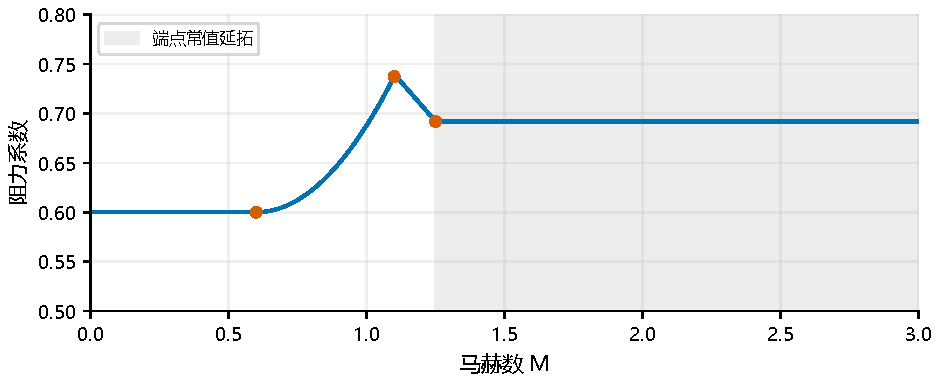
\includegraphics[width=.92\linewidth]{figures/process_q1_drag.pdf}
\caption{采用的阻力系数。灰区为$M>1.25$的常值延拓，节点对应分段边界。}\label{fig:q1-drag}
\end{figure}

中心姿态下$A_{\rm eff}=A$，面积由第5.1.2节标定。气动过载和动压分别定义为
\begin{equation}
 n_D=\frac{D}{mg_0},\qquad q=\frac12\rho v^2.
 \label{eq:load}
\end{equation}
$n_D$表示非重力气动力对应的比力；轨迹的净加速度为$g(h)-n_Dg_0$。匀速下降时$n_D\approx1$，自由落体初期$n_D\approx0$。动压用于计算力和力矩，在本文最大高度搜索中不设置独立动压上限。

\subsubsection{空气动力加热}
速度增加时，近壁气体因压缩与黏性耗散而升温。取定压比热$c_p=\gamma R/(\gamma-1)$，其数值为1004.685\,J/(kg\,K)。滞止温度与恢复温度为
\begin{equation}
 T_0=T+\frac{v^2}{2c_p},\qquad
 T_{\rm aw}=T+r_T\frac{v^2}{2c_p},\qquad
 r_T=\Pr^{1/3},\quad\Pr=0.71.
 \label{eq:heat}
\end{equation}
湍流恢复因子$\Pr^{1/3}$可见NASA-CR-138747的式71\cite{thermal}，本文取$r_T=0.892112$。$T_0$描述完全气体绝热减速至静止的温度，$T_{\rm aw}$描述相应恢复系数下的绝热壁参考温度。它们具有不同的物理意义，均属于气动环境指标。

若实际壁面温度为$T_s$，对流热流还需由换热系数和$T_{\rm aw}-T_s$确定，壁温演化又受热容量、辐射与隔热结构影响。本文选择$T_{\rm aw}\le400$\,K作为装备筛选条件，同时输出$T_0$供对照。400\,K不作为人体温度上限，也不从某种纤维的工业耐热温度直接推导。为区分短峰值与持续暴露，对任一指标$X$定义
\begin{equation}
 \Delta t_{X>X_c}=\int_{t_a}^{t_b}\mathbf 1\{X(t)>X_c\}\,\mathrm dt,
 \label{eq:exposure}
\end{equation}
并记录最长连续超阈区间。数值上在输出点之间线性插值确定阈值穿越时刻。

\subsection{自由降落时的姿态运动}
\subsubsection{刚体方程与简化几何}
姿态运动由角动量平衡决定。在刚体主轴系中，完整方程可写为
\begin{equation}
 \mathbf I\dot{\boldsymbol\omega}
 +\boldsymbol\omega\times(\mathbf I\boldsymbol\omega)
 =\boldsymbol\tau_{\rm aero}+\boldsymbol\tau_{\rm control}.
 \label{eq:euler}
\end{equation}
均匀重力通过质心，不单独产生关于质心的力矩。气动力矩需要给出方向、作用力臂与转动惯量，竖直阻力的时间积分本身不能确定角速度。

本文采用可求解的两自由度简化。$\theta$为腹部朝下参考姿态的俯仰偏角，$\psi$为绕近似竖直下降轴的平旋角。以长$L=1.9$\,m、宽$W=0.6$\,m的均匀薄板表示人体装备的惯量量级：
\begin{equation}
 I_p=\frac{mL^2}{12}=57.158\;\mathrm{kg\,m^2},\qquad
 I_z=\frac{m(L^2+W^2)}{12}=62.858\;\mathrm{kg\,m^2}.
 \label{eq:inertia}
\end{equation}
数值对应190\,kg。这两个惯量固定在参考构型；忽略式\eqref{eq:euler}中两轴间的陀螺耦合，以分析典型扰动和阻尼效应。大角度翻滚与完整三维姿态控制不在这一近似内。

2017年文献给出人体不同方向的投影面积，其中两方向面积比为$\kappa=0.525/1.19$\cite{guerster}。只取这一几何比值，绝对面积使用标定值，令
\begin{equation}
 A_{\rm eff}(\theta)=A\sqrt{\cos^2\theta+\kappa^2\sin^2\theta}.
 \label{eq:area}
\end{equation}
该表达式使姿态变化与平移方程相连，并在参考姿态处恢复$A$。

\subsubsection{恢复力矩、平旋力矩与阻尼}
以$C_\theta$表示俯仰恢复系数，$C_n$表示侧向流动或形状不对称引起的净平旋力矩系数，$C_\omega$表示角阻尼系数，定义
\begin{equation}
 B_\omega=\frac12\rho|v|AL^2C_\omega.
\end{equation}
于是角运动满足
\begin{align}
 \dot\theta&=\omega_p,&
 I_p\dot\omega_p&=-qALC_\theta\sin(2\theta)-B_\omega\omega_p,
 \label{eq:pitch}\\
 \dot\psi&=\omega_z,&
 I_z\dot\omega_z&=qALC_n-B_\omega\omega_z.
 \label{eq:spin}
\end{align}
$B_\omega$的量纲为N\,m\,s，两项阻尼力矩均消耗转动能。平旋驱动力矩$qALC_n$代表绕下降轴的气动不对称；单纯竖直阻力的偏心作用不能直接产生该轴力矩。

中心参数取$C_\theta=0.05,C_n=0.002,C_\omega=0.5$，初始$\theta=0,\omega_p=0,\psi=0,\omega_z=0.05$\,rad/s。这些系数为典型设计假设，不从历史平旋记录拟合。另扫描初始俯仰角5°、15°、30°，$C_n=0,0.002,0.01,0.03$及$C_\omega=0.25,0.5,1$。以头部到旋转轴的距离$r_h=0.5$\,m，取
\begin{equation}
 n_r=\frac{r_h\omega_z^2}{g_0}
 \label{eq:spinload}
\end{equation}
作为头部径向载荷幅值。该量用于工况比较；其沿人体轴线的具体分量还取决于姿态和旋转轴位置。

\subsection{降落伞开启及开启后的下降运动}
\subsubsection{有限时间充气}
令$t_o$为到达$h_o=2566.8$\,m的时刻，$u=(t-t_o)/\tau$。采用首尾导数均为零的平滑充气函数
\begin{equation}
 S(u)=\begin{cases}0,&u\le0,\\3u^2-2u^3,&0<u<1,\\1,&u\ge1.\end{cases}
 \label{eq:inflation}
\end{equation}
取伞衣独立阻力面积$B_c=C_{D,c}A_c$，保留人体阻力，伞降方程为
\begin{equation}
 \dot h=-v,\qquad
 \dot v=g(h)-\frac{\rho v|v|}{2m}\big[C_D(M)A+B_cS(u)\big],
 \qquad n_o=\frac{D+D_c}{mg_0}.
 \label{eq:canopy}
\end{equation}
开伞时高度和速度连续。充气函数控制伞衣有效气动面积的增长，不能直接视为伞衣几何半径的时间规律。开伞阶段固定人体参考面积$A$，表示完成稳定动作后的姿态。

\subsubsection{伞参数与着陆设计}
Airborne Systems的T-11产品资料给出的181.4\,kg载荷下降速度小于18\,ft/s，约为5.49\,m/s，充气时间约6\,s\cite{t11}。本文参考这一量级，为190\,kg系统选择海平面平衡下降速度$v_d=5.5$\,m/s，并重新确定所需阻力面积，不直接套用该型号的承载资格。

低速下$C_D=0.6$，海平面平衡条件给出
\begin{equation}
 B_c=\frac{2mg_0}{\rho(0)v_d^2}-0.6A=\CanopyB\;\mathrm{m^2}.
 \label{eq:canopysize}
\end{equation}
减去$0.6A$是因为人体仍贡献阻力，式\eqref{eq:canopy}分别计入两部分。取等效伞阻力系数$C_{D,c}=1.5$，得到$A_c=\CanopyArea$\,m$^2$；这一系数与面积分解属于伞具设计假设，动力学直接使用$B_c$。中心充气时间为8\,s，4\,s为较快充气对照，后续从载荷约束反求可接受的充气时间。

\section{模型求解与检验}
\subsection{参数标定与检验}
\subsubsection{大气参数的适用性检验}
标准大气提供统一的参考环境，但具体跳跃日的大气会偏离该剖面。本文使用Wyoming探空档案的Santa Teresa站（72364）和Albuquerque站（72365），包括2012年3月15日、7月25日12 UTC，以及10月14日12 UTC和15日00 UTC，共8组探空\cite{wyoming}。由观测压力和温度重新计算密度，比较时统一使用位势高度。重复高度的观测取均值，温度作线性插值，压力作对数线性插值；仅在观测覆盖范围内比较。

图\ref{fig:q1-atmosphere}展示标准剖面及10月14日两站的观测。表\ref{tab:atmcheck}列出8组剖面在10、20、25\,km处的密度相对偏差范围，共24个比较值。偏差定义为$(\rho_{\rm obs}/\rho_{\rm std}-1)\times100\%$。20\,km处的偏差相对较大，表明标准大气近似带来的误差应与气动参数误差共同考虑。
\begin{figure}[htbp]\centering
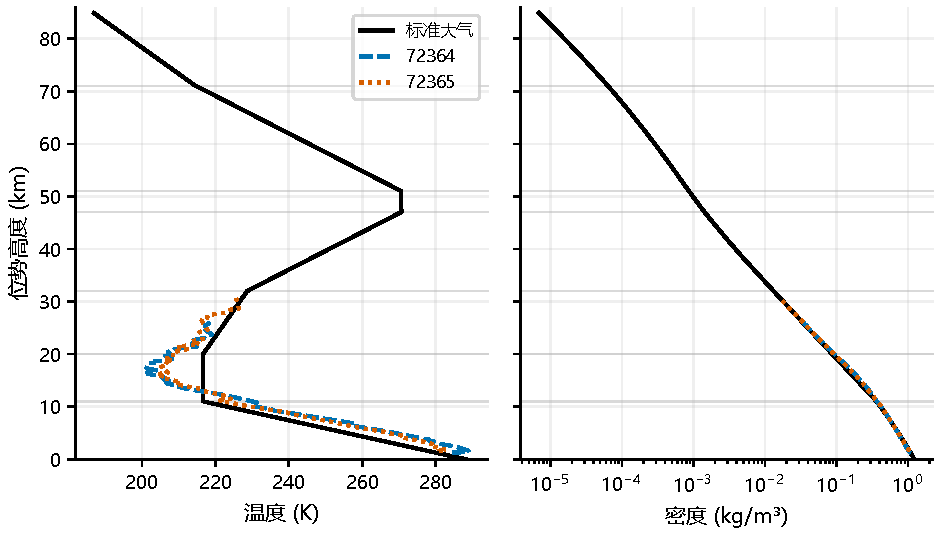
\includegraphics[width=\linewidth]{figures/raw_q1_atmosphere.pdf}
\caption{标准大气与2012年10月14日12 UTC两站探空对比。横向细线对应标准大气位势层界；观测线只画到实际探测高度。}\label{fig:q1-atmosphere}
\end{figure}
\begin{table}[htbp]\centering\small
\caption{8组探空在三个参考位势高度处的密度偏差范围}\label{tab:atmcheck}
\begin{tabular}{rrr}\toprule
位势高度/km & 最小偏差/\% & 最大偏差/\%\\\midrule
\input generated/atmosphere_check.tex 
\bottomrule\end{tabular}
\end{table}

进一步将10月的4组探空分别代入运动方程，保持面积不变。在每组观测的上下边缘设置2\,km平滑过渡带，温度线性混合、压力对数混合，观测范围外继续使用标准大气。图\ref{fig:q1-weather}右图显示，峰速相对标准剖面的变化为0--0.361\,m/s。该结果只反映已观测高度内的替换：72364站14日12 UTC的最高位势高度为25.971\,km，低于模型峰速位置，其零变化与覆盖范围有关，不能由此推断更高空的天气没有影响。
\begin{figure}[htbp]\centering
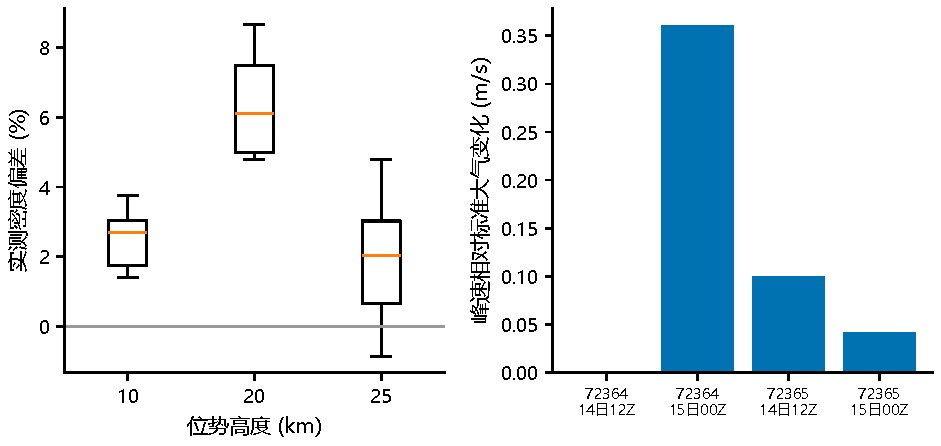
\includegraphics[width=\linewidth]{figures/result_q1_weather.pdf}
\caption{大气检验与局部天气替换的响应。左图每组含8个密度偏差值，箱体表示四分位区间，中线为中位数，须线按1.5倍四分位距确定；右图为4组有限高度探空替换引起的峰速变化。}\label{fig:q1-weather}
\end{figure}

\subsubsection{利用已有高空跳伞数据对迎风面积的标定}
采用3月与7月跳跃的公开峰速及出舱高度\cite{summit}。标定阶段统一取$m_{\rm ref}=121.2$\,kg、固定$C_D=0.6$，只调整面积$A$。设第$j$次跳跃的模型峰速为$V_j(A)$，公开峰速为$V_j^{\rm obs}$，最小化
\begin{equation}
 J(A)=\sum_{j\in\{3\text{月},7\text{月}\}}
 \left(\frac{V_j(A)-V_j^{\rm obs}}{V_j^{\rm obs}}\right)^2.
 \label{eq:calibration}
\end{equation}
相对误差形式使两次不同速度量级的观测都能参与拟合。3月单独反演的面积为1.3355\,m$^2$，7月为1.3893\,m$^2$。联合最优值为$A=\FitArea$\,m$^2$，目标函数约$8.2673\times10^{-5}$。该面积是选定参考姿态和阻力口径下的等效迎风面积，包含姿态与环境简化带来的影响。

表\ref{tab:flights}和图\ref{fig:q1-flights}比较了三次飞行。联合面积使3月和7月峰速误差分别为$-0.58\%$和$+0.70\%$。初始低于0.1\,$g_0$的时间没有参与标定，对7月的预测偏差较明显，说明两个峰速拟合良好并不意味着完整运动过程已被充分确定。正式预测转入式\eqref{eq:drag}的变马赫数阻力，迁移到190\,kg时保持$A$不变并重新积分。
\begin{table}[htbp]\centering\small
\caption{历史跳跃的峰速与初始低过载时间比较。3月和7月用于标定，10月用于检验；时间列为公开值/模型值。}\label{tab:flights}
\begin{tabular}{lrrrrr}\toprule
日期 & 高度/km & 峰速观测 & 峰速模型 & 误差/\% & 低$g$时间/s\\
 & & \multicolumn{2}{c}{m/s} & & \\\midrule
\input generated/flights.tex 
\bottomrule\end{tabular}
\end{table}
\begin{figure}[htbp]\centering
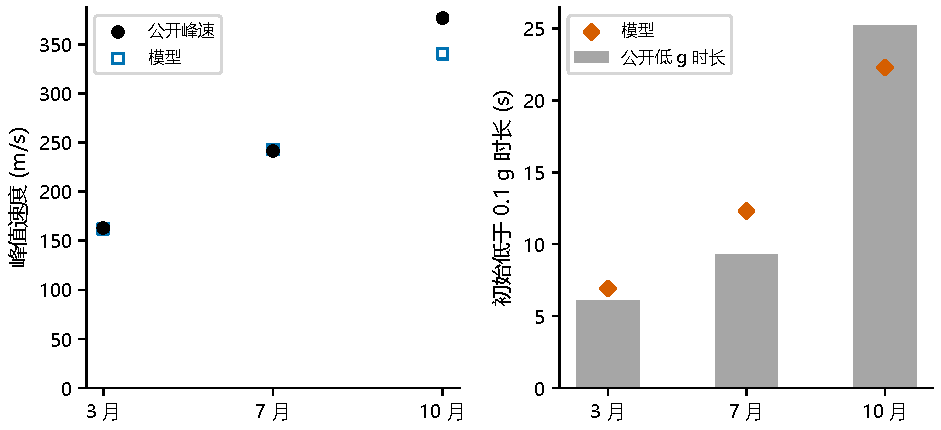
\includegraphics[width=\linewidth]{figures/raw_q1_flights.pdf}
\caption{三次跳跃的峰速与初始低过载时长。3月、7月峰速用于面积标定，低过载时长及10月数据用于比较。}\label{fig:q1-flights}
\end{figure}

\subsubsection{利用已有高空跳伞数据对模型的检验}
10月出舱高度为38969.4\,m，公开峰速为377.1\,m/s。面积沿用联合标定值，模型峰速为\OctV\,m/s，低估\OctError\%；峰速出现时间为47.11\,s，文献约50\,s；模型峰速高度为29.306\,km。2017年论文记载的峰速高度为28.833\,km，峰会报告另记27.833\,km，本文与2017年图线比较时采用前者，并保留这一来源差异\cite{guerster,summit}。

为了检验整段轨迹，从2017年论文图1的原始嵌入图像中提取速度实线。图像尺寸为1782$\times$1102像素；用35、30、25、20、15\,km五个横轴刻度拟合线性高度映射，用0、400\,m/s两个纵轴刻度建立速度映射。每隔4列在人工核对的走廊中读取黑色线条中心，得到411点；被其他图线遮盖的一列跳过，未补造该处观测。有效高度范围为12.969--38.737\,km。

以$\pm3$像素作为读取半宽，对应约$\pm47$\,m和$\pm1.39$\,m/s。这是本次图线读取分辨率，未包含原数据处理误差；2017年论文对速度数字化误差另估约5\%。411个图线上点互有相关性，不能视为411次独立实验。比较时将模型速度插值到这些高度，定义
\begin{equation}
 e_i=v_{\rm mod}(h_i)-v_{\rm obs}(h_i),\quad
 \mathrm{RMSE}=\sqrt{\frac1N\sum_i e_i^2},\quad
 \mathrm{MAE}=\frac1N\sum_i|e_i|.
 \label{eq:error}
\end{equation}
图\ref{fig:q1-validation}给出实测图线与模型的$v$--$h$比较和残差。RMSE为\CurveRMSE\,m/s，MAE为\CurveMAE\,m/s，平均偏差为\CurveBias\,m/s，最大绝对偏差为\CurveMax\,m/s。模型在高速及减速阶段总体低估速度，可能与三次跳跃的有效姿态差别、统一参考质量和标准大气近似有关。

\begin{figure}[htbp]\centering
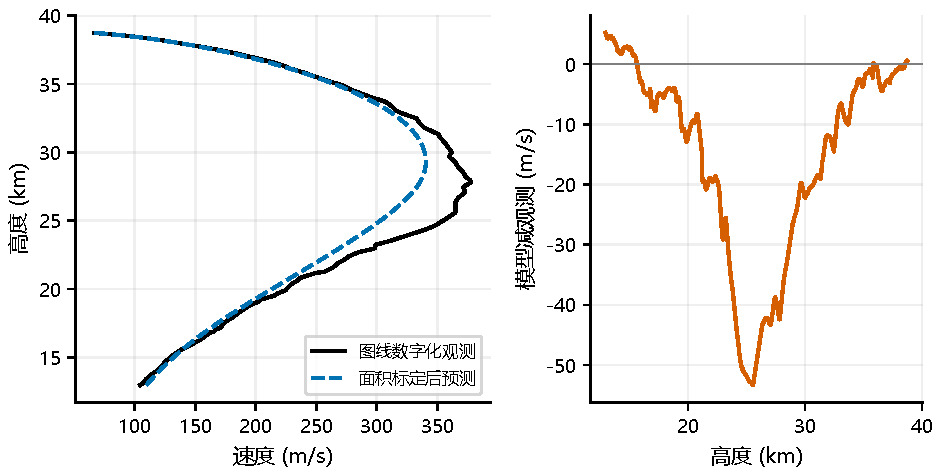
\includegraphics[width=\linewidth]{figures/result_q1_validation.pdf}
\caption{10月跳跃的速度—高度检验。左图黑线为2017年图1数字化观测，蓝色虚线为固定联合面积下的预测；右图为模型减观测的速度残差。}\label{fig:q1-validation}
\end{figure}

10月数据未用于面积再拟合，但阻力公式本身由10月飞行推导。因此这里是对面积迁移及简化动力学的同源检验，其误差应进入模型评价，不能作为完全独立的高空极限验证。

\subsection{模型求解与讨论}
\subsubsection{音障}
对190\,kg系统数值求解式\eqref{eq:motion}及角运动方程，并以到达开伞高度和地面作为阶段终止事件。图\ref{fig:q1-trajectory}左图比较40--80\,km出舱的速度剖面；右图给出中心最大高度工况的速度、声速和局部收尾速度。稀薄高空首先允许较长时间加速，随后密度增长使阻力迅速增加，速度转为下降。

\begin{figure}[htbp]\centering
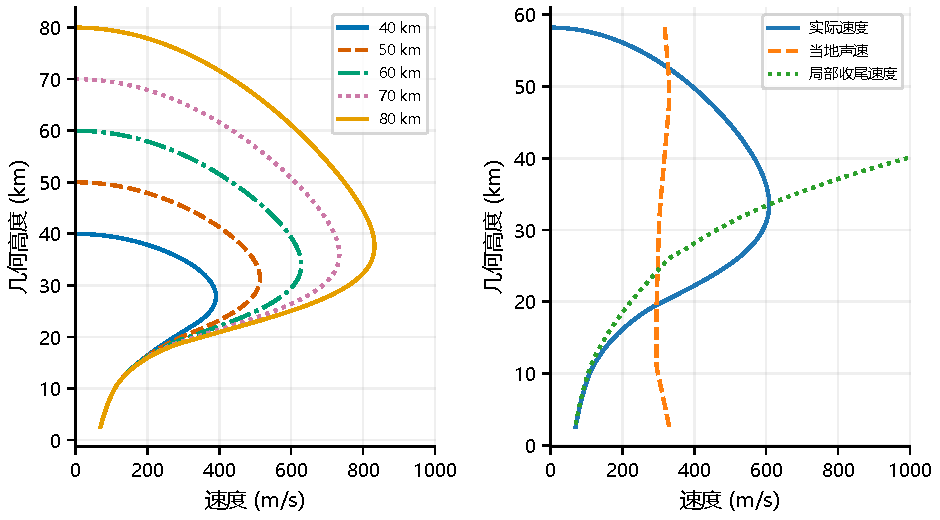
\includegraphics[width=\linewidth]{figures/process_q1_trajectory.pdf}
\caption{不同出舱高度的速度剖面及临界工况的速度尺度。右图的局部收尾速度由当地力平衡求得，高空部分超出横轴显示范围。}\label{fig:q1-trajectory}
\end{figure}

中心边界工况在出舱后\FirstSonic\,s首次达到$M=1$，在\LastSonic\,s降回亚声速，超声速持续\SuperTime\,s，峰值马赫数为\PeakMach。跨越声速会改变压缩性阻力和局部流场，但一维方程在$M=1$附近没有奇点；音障本身不是本文单独设置的失败条件。实际影响通过阻力系数、热指标和姿态力矩体现。中心工况最高马赫数接近2，已进入经验阻力公式的延拓段，是结果的不确定性来源之一。

\subsubsection{收尾速度}
本文将固定高度、固定姿态下重力与阻力平衡的速度称为局部收尾速度，也称终端速度。它满足
\begin{equation}
 m g(h)=\frac12\rho(h) C_D\!\left(\frac{v_t}{c(h)}\right) A_{\rm eff}v_t^2.
 \label{eq:terminal}
\end{equation}
若$C_D$固定，可得$v_t=\sqrt{2mg/(\rho C_DA_{\rm eff})}$；采用变马赫数阻力时需数值求根。由于密度随高度不断变化，实际速度通常无法始终跟随这一局部平衡值。实际速度超过$v_t(h)$时进入减速，接近低空后则逐渐追随下降中的收尾速度曲线。

原始$C_D$系数在$M=1.1$的舍入跳跃可能使极少数高度的精确力平衡根缺失；绘图程序在此留空，未将跳跃点误当成零残差根。低空开伞前各条轨迹趋于相近，这解释了较高出舱情景在同一开伞高度附近得到几乎相同的开伞速度与载荷。

\subsubsection{最大高度搜索与阈值敏感性}
定义出舱高度$h_0$的可行集合
\begin{equation}
\mathcal H=\left\{h_0:\begin{array}{l}
\max n_D\le5,\quad\max n_o\le5,\\
\max T_{\rm aw}\le400\;\mathrm K,\quad\max n_r\le2,\\
v_{\rm land}\le6\;\mathrm{m/s}
\end{array}\right\},\qquad H_{\max}=\sup\mathcal H.
\label{eq:feasible}
\end{equation}
自由段和开伞段分别求峰值；角载荷取自由下降阶段。扫描从0.1\,km开始，随后以1\,km间隔覆盖至86\,km。零高度为无下降的退化边界，不影响最大值搜索。对各约束相邻扫描点的符号变化进行括区间，再用Brent方法细化，求根高度容差为0.05\,m，同时检查各区间内部的可行性。

图\ref{fig:q1-limits}将各指标除以对应设计上限。中心可行区间的上界为\MaxHeight\,km，此时恢复温度达到400\,K；其他单项约束在0.1--86\,km扫描内均未单独触及上界。因此，只能说这些约束在本范围内不主导，不能把86\,km解释为它们的临界高度。
\begin{figure}[htbp]\centering
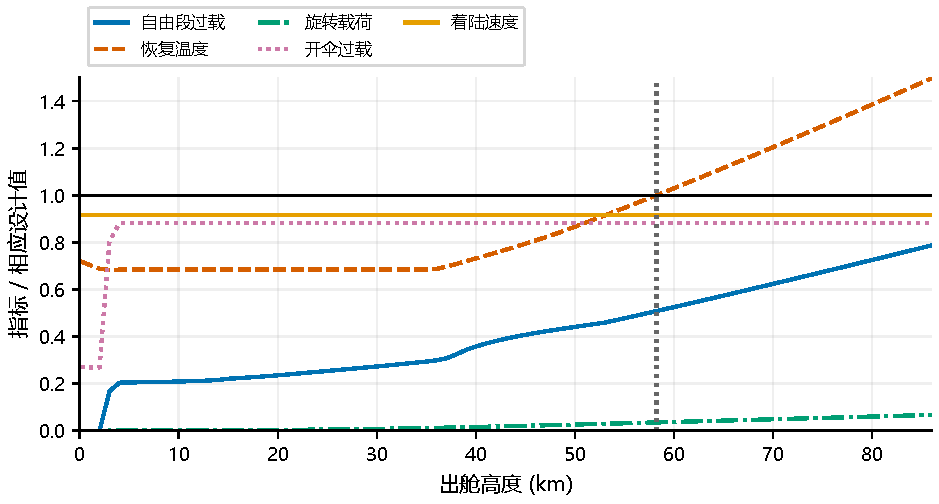
\includegraphics[width=\linewidth]{figures/result_q1_limits.pdf}
\caption{中心设计条件下各指标随出舱高度的变化。水平实线为归一化上限1，竖虚线对应约\MaxHeight\,km的联合边界。}\label{fig:q1-limits}
\end{figure}

典型高度的结果见表\ref{tab:cases}。提高出舱高度会显著增加峰速、热指标和自由段过载，中心旋转载荷也随之上升。表\ref{tab:sensitivity}给出每次只改变一个筛选上限的结果：恢复温度上限由380增至420\,K时，最大高度从55.21增至61.18\,km；若开伞上限降到4\,$g_0$，高空情景受开伞约束排除，保留的上界仅约2.99\,km。
\begin{table}[htbp]\centering\small
\caption{190\,kg系统在不同出舱高度下的自由下降峰值}\label{tab:cases}
\begin{tabular}{rrrrrr}\toprule
$h_0$/km & $v_{\max}$/(m/s) & $M_{\max}$ & $\max n_D$ & $\max T_{\rm aw}$/K & $\max n_r$\\\midrule
\input generated/cases.tex 
\bottomrule\end{tabular}
\end{table}
\begin{table}[htbp]\centering\small
\caption{单项设计上限变化对联合最大高度的影响；斜线分隔值一一对应}\label{tab:sensitivity}
\begin{tabularx}{\linewidth}{p{34mm}p{39mm}Y}\toprule
改变的上限 & 取值 & 联合最大高度/km\\\midrule
\input generated/sensitivity.tex 
\bottomrule\end{tabularx}
\end{table}
严格采用5.5\,m/s着陆上限时，扫描中没有可行点，是因为着地时尚有微小动态滞后，实际速度约5.5004\,m/s，比海平面静态平衡设计值大约0.0004\,m/s。这一数值边界不表示装备性能出现突变，中心方案采用6\,m/s筛选值。

把面积分别取为3月、联合、7月标定值，重新计算400\,K热边界，得到表\ref{tab:areas}。这一小范围变化对应约58.16--58.32\,km，不应视为统计置信区间；它只衡量两次峰速标定差异，未包括10月所揭示的模型系统偏差。
\begin{table}[htbp]\centering\small
\caption{面积标定方案与相应400\,K热边界。March、joint、July分别表示3月、联合及7月标定。}\label{tab:areas}
\begin{tabular}{lrr}\toprule
标定方案 & $A$/m$^2$ & 热边界/km\\\midrule
\input generated/area.tex 
\bottomrule\end{tabular}
\end{table}

\subsubsection{数值检验与极值位置}
积分采用自适应Runge--Kutta方法，自由段最大步长0.5\,s，伞段0.25\,s，相对容差$10^{-8}$；利用连续输出在采样极值附近局部优化。表\ref{tab:peaks}给出边界工况各峰值的位置，表明速度、热、载荷峰值并不同步。
\begin{table}[htbp]\centering\small
\caption{\MaxHeight\,km中心工况的自由下降极值及其出现位置}\label{tab:peaks}
\begin{tabular}{lrrr}\toprule
指标 & 峰值 & 出舱后时间/s & 几何高度/km\\\midrule
\input generated/peaks.tex 
\bottomrule\end{tabular}
\end{table}

物理检验包括七层大气基准值及连续性、静力平衡差分关系、阻力系数端点、真空变重力能量守恒、恒定重力与密度下的解析收尾速度、无外力矩时角动量守恒、气动阻尼符号及伞降地面事件。恒定环境解析解使用$v=v_t\tanh(gt/v_t)$与生产求解方程对照。将两阶段最大步长缩小至0.05\,s、相对容差收紧至$10^{-10}$后，边界工况各风险峰值相对差小于$3\times10^{-7}$；更精细热边界求解的高度差为\HeightConvergence\,m。数值离散误差远小于气动参数和筛选条件带来的差异，正文最终高度取两位小数已足够。

\section{危险性分析}
\subsection{自由降落过载}
自由下降的危险载荷应与人体感受到的比力对应。式\eqref{eq:load}中的$D/m$为气动力加速度，速度方程中的$\dot v$还包含重力项。中心工况自由段峰值为\FreeG\,$g_0$，约在出舱后91.59\,s、几何高度23.265\,km出现，超过5\,$g_0$的持续时间为零。图\ref{fig:q1-heating}左图显示过载先增大再趋近低空准平衡值。

\begin{figure}[htbp]\centering
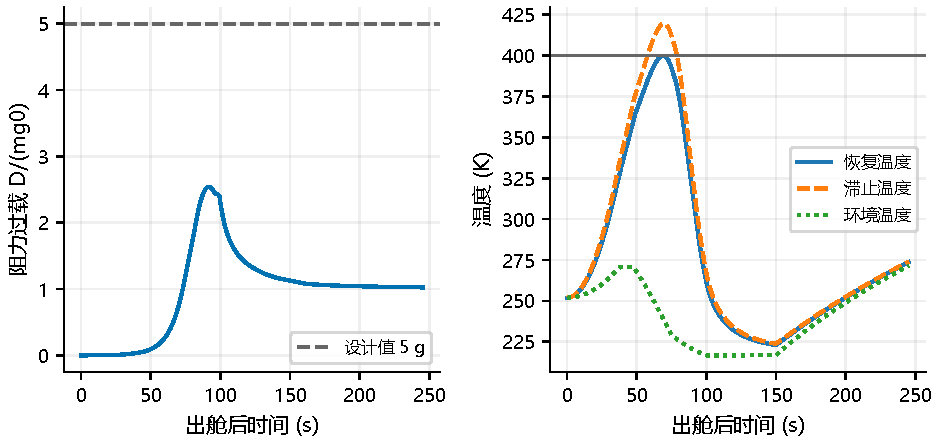
\includegraphics[width=\linewidth]{figures/process_q1_heating.pdf}
\caption{\MaxHeight\,km中心工况的自由段过载与热过程。左图虚线为5\,$g_0$设计值，右图水平线为400\,K恢复温度上限。}\label{fig:q1-heating}
\end{figure}

过载方向会随姿态和约束方式改变。腹部朝下的分布式气动力、伞带传力和头部旋转载荷的受力路径不同，不能用一个历史峰值覆盖所有阶段。本文分别计算自由段、开伞段及旋转幅值，并保留各自的时间信息。当前中心情景中，自由段载荷低于热边界处的筛选值，因此不先于热约束决定最大高度。

\subsection{高温危险}
图\ref{fig:q1-heating}右图显示，边界工况的恢复温度在出舱后约68.94\,s、几何高度35.922\,km达到400\,K；滞止温度的峰值为\Tzero\,K。热峰比过载峰出现更早，因为热指标主要与$v^2$及当地气温有关，阻力则还随大气密度强烈变化。

从60、70、80\,km出舱时，恢复温度超过400\,K的持续时间分别为\SixtyHeatTime\,s、\SeventyHeatTime\,s和\EightyHeatTime\,s。高度增加不仅抬高峰值，也延长超阈暴露。中心边界在数值精度内恰好触及上限，物理意义是当前热筛选条件的临界情景。

热防护优化需要同时考虑面罩、密封件、压力服外层及隔热层，不能只依据一个材料耐温值判断整个系统。本文的380--420\,K敏感性区间用来显示设计要求变化的影响，未将其解释为人体可接受温度区间。

\subsection{旋转危险}
图\ref{fig:q1-attitude}左图给出初始俯仰扰动的演化。稀薄空气中的恢复与阻尼很弱，姿态变化较慢；进入较稠密大气后产生阻尼振荡，最终回到参考姿态。初始偏角从5°增加到30°时，中心高度的峰值恢复温度变化不到0.1\,K，说明在所选恢复力矩下，小到中等俯仰扰动能够较快衰减。此结论依赖恢复系数的正值和固定参考惯量近似。
\begin{figure}[htbp]\centering
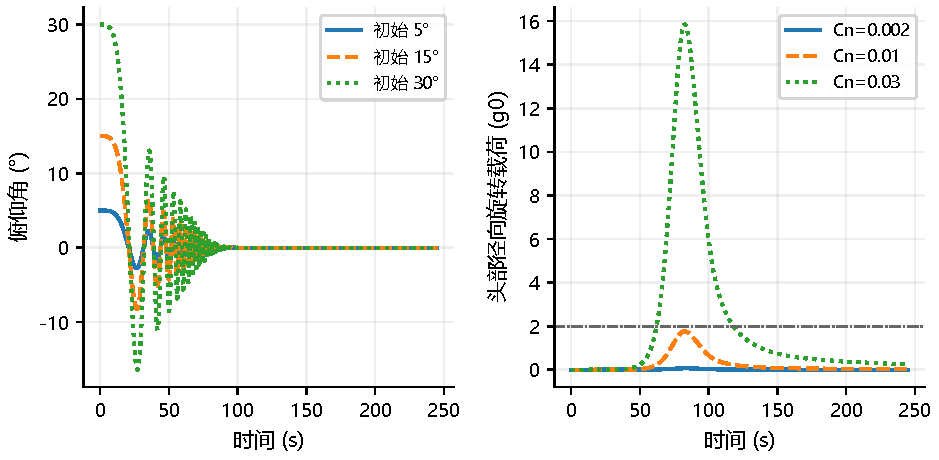
\includegraphics[width=\linewidth]{figures/process_q1_attitude.pdf}
\caption{中心高度下的姿态扰动。左图比较5°、15°、30°初始俯仰角；右图固定$C_\omega=0.5$，比较三种平旋偏置力矩系数引起的头部径向载荷。}\label{fig:q1-attitude}
\end{figure}

平旋对应不同的受力机制。中心$C_n=0.002,C_\omega=0.5$情景的峰值角速度约11.24\,rpm，头部径向载荷为\SpinG\,$g_0$。当$C_n$增至0.01时，峰值约56.13\,rpm、1.76\,$g_0$；当$C_n=0.03,C_\omega=0.25$时，模型给出约50.70\,$g_0$的高旋转载荷，已远超设计条件。该极端结果说明力矩不对称与阻尼不足能够改变风险排序；它是简化模型的参数情景，未证明真实人体存在对应的稳定性分岔或可达到该角速度。

\begin{figure}[htbp]\centering
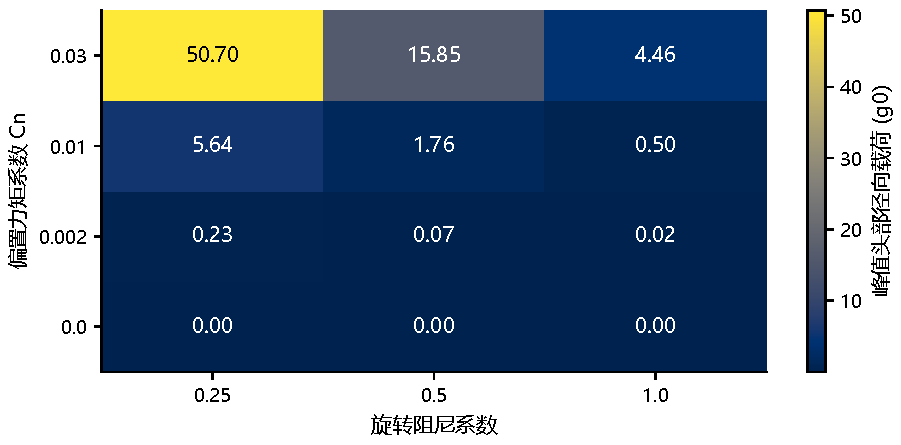
\includegraphics[width=\linewidth]{figures/result_q1_spin_sensitivity.pdf}
\caption{平旋偏置和阻尼敏感性。单元格为中心出舱高度下的峰值头部径向载荷，单位$g_0$；各组合为设计参数扫描。}\label{fig:q1-spin}
\end{figure}

图\ref{fig:q1-spin}表明，增强角阻尼或降低形状不对称可有效减小旋转载荷。Stratos峰会报告记载10月平旋约持续13\,s、最高不超过60\,rpm、头部载荷低于2\,$g_0$\cite{summit}，可作为工况量级对照。报告中的腕部3.5\,$g_0$持续6\,s是自动稳定伞触发设置，本文未将其当作人体耐受极限。实际防护仍需姿态控制、稳定伞和传感触发策略的配合，且必须考虑触发位置与人体轴向载荷的差别。

\subsection{开伞过载}
中心工况到达开伞高度时的速度为\OpenV\,m/s。图\ref{fig:q1-opening}显示，充气时间改变会显著影响载荷峰值。8\,s充气的峰值为\OpenG\,$g_0$，约在拉伞后1.23\,s出现；4\,s充气的峰值为\FastOpenG\,$g_0$，超过5\,$g_0$约\FastOverTime\,s。充气时间并不等于载荷峰值出现时间，因为有效面积增长和速度下降同时发生。
\begin{figure}[htbp]\centering
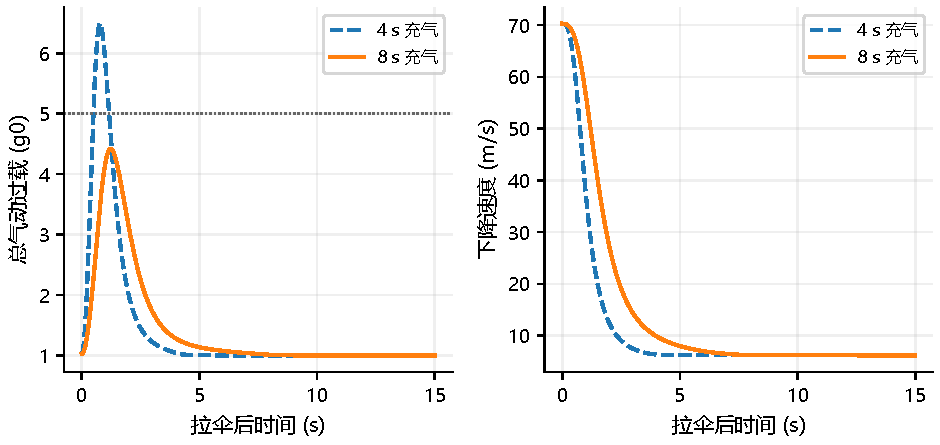
\includegraphics[width=\linewidth]{figures/process_q1_opening.pdf}
\caption{相同开伞高度与入流速度下，4\,s和8\,s充气的总气动过载及速度响应。载荷包含人体与伞衣两部分。}\label{fig:q1-opening}
\end{figure}

在当前平滑充气函数、伞阻力面积和入流条件下，反求满足5\,$g_0$峰值限制的最小充气时间约为\MinimumInflation\,s。8\,s方案满足这一条件，4\,s方案不满足。由于高空出舱轨迹在主伞高度已接近相同收尾速度，继续增加出舱高度对该处开伞载荷的影响很小；因此，开伞是否可行主要取决于低空空速与充气设计。

该分析尚未描述伞绳弹性、收口机构、伞衣呼吸和不对称展开。设计缓慢展开时，还须检查充气期间的高度损失与备份伞需求。本文以连续地面事件确认所选8\,s方案有足够下降高度，不能将光滑阻力函数直接作为实际伞具认证结果。

\subsection{着陆}
8\,s充气方案的着陆速度约\LandingV\,m/s，伞下降落时间约\ChuteTime\,s，自由阶段约\FreeTime\,s，全程约\TotalTime\,s。生命保障必须覆盖完整过程，并留出实际操作裕量。着陆时系统竖直动能为
\begin{equation}
 E_k=\frac12mv_{\rm land}^2\approx\Energy\;\mathrm{kJ}.
\end{equation}
若用有效压缩行程$s_b$吸收动能，按恒定平均净减速度近似，有
\begin{equation}
 a_{\rm net}=\frac{v_{\rm land}^2}{2s_b},\qquad
 \frac{N}{mg_0}=1+\frac{v_{\rm land}^2}{2s_bg_0},
 \label{eq:landing}
\end{equation}
其中$N$为平均地面支承力。缓冲行程0.3、0.5、0.8\,m时，归一化支承载荷约为6.14、4.09、2.93。若以5\,$g_0$平均支承载荷为设计值，则至少需要约\Stroke\,m有效行程。人体屈膝动作、着陆翻滚及缓冲结构可共同提供行程，实际瞬时峰值取决于力—位移曲线。着陆面坡度、水平风速和触地姿态尚需在具体装备设计中补充。

\section{结论}
本文对190\,kg太空跳伞系统建立了分层大气下的平移—姿态动力学、气动热指标和有限时间开伞模型。3月、7月历史峰速在固定$C_D=0.6$下给出联合面积\FitArea\,m$^2$；10月检验的峰速低估\OctError\%，整段速度—高度曲线RMSE为\CurveRMSE\,m/s，说明所选简化对历史飞行具有明确且可量化的偏差。

采用400\,K恢复温度、5\,$g_0$自由与开伞过载、2\,$g_0$径向载荷、6\,m/s着陆速度上限，以及8\,s充气和中心姿态参数时，\textbf{最大出舱高度约为\MaxHeight\,km}。边界工况峰速\PeakV\,m/s、最高马赫数\PeakMach，自由段过载\FreeG\,$g_0$，开伞过载\OpenG\,$g_0$，最终以约\LandingV\,m/s到达海平面。恢复温度在中心情景中先达到约束，改变其上限到380--420\,K会将最大高度改变为55.21--61.18\,km。

成功下降还取决于开伞与姿态控制：4\,s充气产生\FastOpenG\,$g_0$的峰值载荷，在本文设计条件下不可接受；偏置力矩增加或角阻尼减弱也可能使旋转载荷转为主导风险。因此，提高允许高度需要同步改进热防护、控制气动力矩并限制开伞载荷，单独提高出舱高度不能保证更好的任务结果。

\section{模型评价}
\subsection{模型优点}
大气模型直接使用标准文献的七层温度梯度，通过静力方程推导压力和密度，具有清楚的单位、层界和适用范围。阻力系数、迎风面积及质量分别处理，便于区分经验气动规律、标定信息和190\,kg系统的迁移计算。

模型把自由下降、姿态、热指标、有限充气与着陆连接为完整过程，分别输出峰值、出现位置和暴露时间；最大高度由多项约束的可行区间确定。观测曲线数字化、未参与面积拟合的10月比较及局部天气替换，使模型误差有可追溯依据。解析基准与步长收敛检查则表明，当前答案主要受物理假设影响，数值积分误差较小。

\subsection{模型缺点}
首先，面积只由两次峰速标定，有效姿态差异未被独立识别；10月约9.66\%的峰速低估表明跨跳跃迁移存在系统误差。$M>1.25$使用常值阻力延拓，而中心峰值接近$M=2$，需要更高马赫数的气动数据才能改善该部分预测。

其次，恢复温度尚未转化为压力服的瞬态壁温或人体热负荷，400\,K属于设计筛选条件。两自由度姿态模型采用假设力矩系数和固定惯量，省略主动动作、陀螺耦合与大角度翻滚；高旋转载荷情景主要用于识别参数敏感性。

最后，模型未包含三维风场、地形、真实伞衣与伞绳结构动力学，也未完成190\,kg质量预算下的具体装备设计。今后的改进应优先增加姿态与气动测量、压力服传热参数及分阶段开伞数据，使目前的条件性高度进一步转化为可验证的装备性能指标。

\begin{thebibliography}{9}
\bibitem{problem} University Physics Competition. 2023 Competition Problems: Problem A, Space Diving. 2023. \url{https://www.uphysicsc.com/2023contest.html}.
\bibitem{ussa} NOAA, NASA, USAF. \emph{U.S. Standard Atmosphere, 1976}. Washington, DC, 1976. 印刷页3表4及第6页静力关系. \url{https://ntrs.nasa.gov/citations/19770009539}.
\bibitem{guerster} Guerster M, Walter U. Aerodynamics of a highly irregular body at transonic speeds---Analysis of STRATOS flight data. \emph{PLOS ONE}, 2017, 12(12): e0187798. \url{https://doi.org/10.1371/journal.pone.0187798}.
\bibitem{summit} Red Bull Stratos. \emph{Scientific Summit: Summary Report}. California Science Center, Los Angeles, January 23, 2013. 跳跃汇总、姿态及开伞记录. \url{https://lru.praxis.dk/Lru/microsites/hvadermatematik/hem3download/kap3a_QR20_ekstra_Report_Final.pdf}.
\bibitem{thermal} Chung S. \emph{Survey of literature on convective heat transfer coefficients and recovery factors for high atmosphere thermometry}. NASA-CR-138747, 1973. 印刷页58，式71. \url{https://ntrs.nasa.gov/citations/19740019690}.
\bibitem{hidh} NASA. \emph{Human Integration Design Handbook}, Revision 1. NASA/SP-2010-3407/REV1, 2014, Section 6.5. \url{https://www.nasa.gov/wp-content/uploads/2023/03/human-integration-design-handbook-revision-1.pdf}.
\bibitem{t11} Airborne Systems. \emph{T-11 Personnel Parachute System}, product sheet, 2017, Spanish edition. \url{https://airborne-sys.com/wp-content/uploads/2025/04/ASG-T-11-20170202-Spanish.pdf}.
\bibitem{wyoming} University of Wyoming. Upper Air Soundings Archive. 站点72364、72365，2012年3月15日、7月25日、10月14--15日记录. \url{https://weather.arcc.uwyo.edu/upperair/sounding.shtml}.
\end{thebibliography}
\end{document}


